\documentclass{standalone}
\usepackage{tikz}
\usepackage[]{xcolor}
\usetikzlibrary{calc}
\usepackage{bbold}
\usepackage{physics}

\newcommand{\mcG}{\mathcal{G}}

\graphicspath{{../figs/}}


\usepackage{amsmath, amsthm, amssymb}
\colorlet{coscolor}{blue}

\newcommand{\red}{\color{red}}
\newcommand{\blue}{\color{blue}}
%Colors

\definecolor{max}{rgb}{1,0.54,0.1}
\definecolor{medium}{rgb}{1,0.8,0.6}
\definecolor{min}{rgb}{1,0.9,0.8}
\begin{document}
\pagestyle{empty}
\newcommand{\tmpa}{7}
\newcommand{\xo}{0}
\newcommand{\separation}{1.02}
\newcommand{\scalefont}{1.1}
\begin{tikzpicture}
\node[anchor=north west] at (\xo, 0) {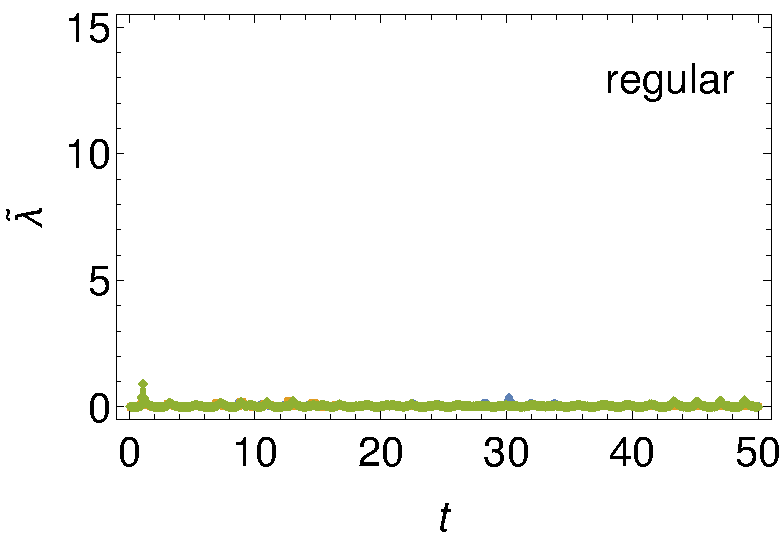
\includegraphics[width=\tmpa cm]{lambda_tilde_choi_regular.pdf}};
\node[anchor=north west] at (\xo \separation*\tmpa, 0)
{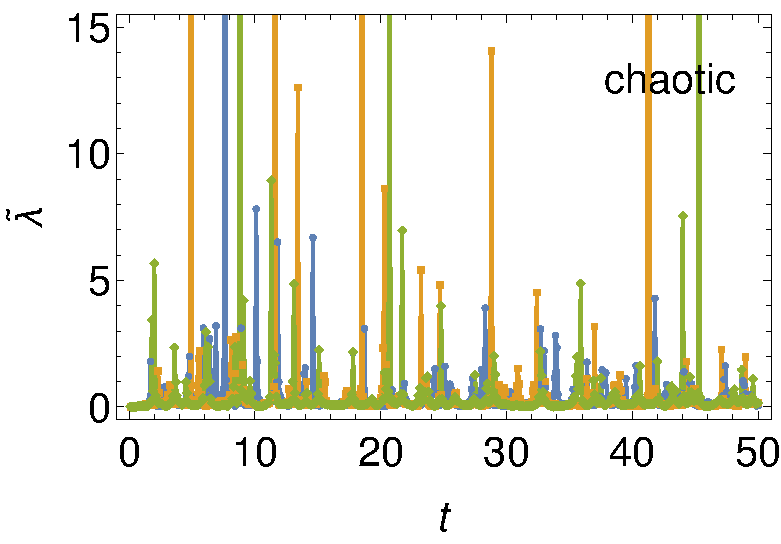
\includegraphics[width=\tmpa cm]{lambda_tilde_choi_chaotic.pdf}};
\node[anchor=north west] at (0, 0) {\scalebox{\scalefont}{(a)}};
\node[anchor=north west] at (\separation*\tmpa, 0) {\scalebox{\scalefont}{(b)}};
\end{tikzpicture}
\end{document}